\section{Introduction}
Computer programming can be found in nearly all parts of society. Spanning entertainment, healthcare, education, and more, programming is an extraordinarily general tool with applications that are vast in scope. As computers are becoming more ubiquitous in modern life, rising demand for high-quality code draws an ever-greater number of aspiring programmers to the profession. After years of study to become proficient coders, human experts are are able to convert abstract specifications of diverse cognitive tasks into concrete programs.

In the past few years, large-scale language models have shown promise in generalizing to various cognitive tasks, including linguistic inference \citep{NEURIPS2019_4496bf24}, commonsense reasoning \citep{zellers2019hellaswag,huang2019cosmosqa,bisk2019physicaliqa}, logical deduction \citep{Liu2020LogiQAAC}, mathematics \citep{Polu2020GenerativeLM,hendrycksmath2021}, and general understanding of multiple domains of human knowledge \citep{hendryckstest2021}. However, whether large-scale language models can reliably write code remains an open question. %

Motivated by the potential of language models and the need for thorough code generation evaluation, we introduce APPS, a benchmark for code generation from natural language specifications. Unlike prior work on code generation with Transformer language models \citep{Vaswani2017AttentionIA}, which mostly focuses on code translation \citep{lachaux2020unsupervised} and pseudocode-to-code \citep{NEURIPS2019_7298332f}, we evaluate models on their ability to take specifications given in natural language and write code that meets these specifications. This setting mirrors how human coders are evaluated and is a more realistic and informative setting in which to benchmark models.

\begin{figure*}[t]
    \centering
    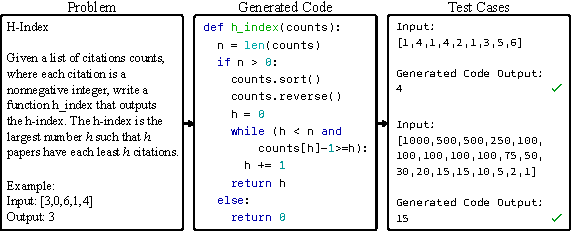
\includegraphics[width=\textwidth]{figures/splash2.pdf}
    \caption{An example problem from APPS (left) along with possible generated code (middle) and two example test cases we use to evaluate the generated code (right). Our evaluation framework has test cases and $10,\!000$ code generation problems of varying difficulty levels.}
    \label{fig:apps_splash}
\end{figure*}

APPS provides a precise and comprehensive view of code generation. APPS evaluates models not only on their ability to code syntactically correct programs, but also on their ability to understand task descriptions and devise algorithms to solve these tasks. It contains $10,\!000$ programming problems at various levels of difficulty, covering simple introductory problems, interview-level problems, and coding competition challenges. If a model were to perform well on APPS, this would indicate an ability to flexibly use data structures and programming techniques, as well as an ability to correctly interpret diverse task specifications, follow instructions, and understand human intent \citep{hendrycks2021ethics}.

For most text generation tasks, high-quality evaluation requires human feedback, which can be time-consuming or carry pecuniary costs. As a result, automatic metrics such as BLEU \citep{papineni2002bleu} are often used to compare methods, but these metrics do not necessarily track program correctness. Since the objective for code generation is to produce correct programs, we assess programs not with BLEU but with test cases and error catching. Evaluating code generation on APPS is facilitated by a large bank of over $130,\!000$ test cases. The test cases are specifically chosen to probe correct functionality across the input space. By using test cases, we provide a gold-standard metric for code generation quality.

In our experiments, we find that models are now starting to exhibit nonzero accuracy and solve some coding problems. Additionally, as models improve, we observe that syntax errors are exponentially decreasing. We also find further evidence that BLEU is a problematic metric for code generation, sometimes being anticorrelated with gold-standard accuracy. We find that accuracy decreases with difficulty level and improves through fine-tuning and model size increases. The strongest model that we evaluate on introductory problems passes almost $20\%$ of test cases given five attempts. These results position code generation as a challenging but now tractable testbed for large-scale language models.

Writing code to meet specifications in natural language is an economically valuable task with widespread social implications should it be solved, as it could eventually facilitate malicious code generation and one day result in job automation. As large-scale language models have the potential to make significant progress on code generation, it is essential that we begin to track advancements on this task. Our new benchmark facilitates measuring performance in an accurate and rigorous manner. Using APPS, we find that programming is very difficult for modern language models, though performance is improving. Thus, the APPS benchmark can provide foresight about the performance of future large-scale language models at the critical task of program synthesis from natural language. The dataset is available at \href{https://github.com/hendrycks/apps}{https://github.com/hendrycks/apps}.







